\PassOptionsToPackage{obeyspaces,spaces}{url}
\PassOptionsToPackage{hidelinks}{hyperref}
\documentclass[11pt,a4paper]{article}

% ---------- Fonts: Arial (metric-compatible Liberation Sans if Arial is not installed). Compile with XeLaTeX. ----------
\usepackage{fontspec}
% Liberation Sans is metrically identical to Arial. To use Arial itself, replace the three names below by
% Arial, Arial and Courier New (the fonts must be installed on the machine that compiles the file).
\setmainfont{Liberation Sans}
\setsansfont{Liberation Sans}
\setmonofont[Scale=MatchLowercase]{Liberation Mono}
\usepackage{microtype}

% ---------- Layout ----------
\usepackage[a4paper,margin=2.5cm]{geometry}
\usepackage{graphicx}
\graphicspath{{../img/}}
\usepackage{booktabs}
\usepackage{tabularx}
\usepackage{array}
\usepackage{enumitem}
\usepackage{caption}
\usepackage{float}
\usepackage{fancyhdr}
\usepackage{longtable}
\usepackage{titlesec}
\usepackage{url}
\urlstyle{tt}


\usepackage{hyperref}
\hypersetup{
  pdftitle={Anti-Fragile Agentic Workflow (AFAW): A Deterministic, Multi-Agent Methodology for AI-Assisted Software Development},
  pdfauthor={Agustin Diaz-Cano},
  pdfsubject={Software engineering methodology for AI-assisted development with multiple coding agents},
  pdfkeywords={AI-assisted development, coding agents, multi-agent, continuous integration, mutation testing, test-driven development, large language models}
}

% ---------- Macros ----------
\newcommand{\code}[1]{\path{#1}}
\newcommand{\afaw}{AFAW}
\newcolumntype{Y}{>{\raggedright\arraybackslash}X}
\setlist{itemsep=2pt, topsep=4pt, parsep=0pt}
\captionsetup{font=small, labelfont={bf,sf}, labelsep=period}
\renewcommand{\arraystretch}{1.18}

\titleformat{\section}{\sffamily\Large\bfseries}{\thesection}{0.7em}{}
\titleformat{\subsection}{\sffamily\large\bfseries}{\thesubsection}{0.7em}{}
\titleformat{\subsubsection}{\sffamily\normalsize\bfseries}{\thesubsubsection}{0.7em}{}

\pagestyle{fancy}
\fancyhf{}
\fancyhead[L]{\small\sffamily AFAW: Anti-Fragile Agentic Workflow}
\fancyhead[R]{\small\sffamily A. Diaz-Cano}
\fancyfoot[C]{\small\sffamily\thepage}
\renewcommand{\headrulewidth}{0.3pt}
\setlength{\headheight}{14pt}

\setlength{\parskip}{4pt}
\setlength{\emergencystretch}{3em}
\setlength{\parindent}{0pt}

% Float placement: allow large figures to take a page of their own without blocking the queue
\renewcommand{\topfraction}{0.9}
\renewcommand{\bottomfraction}{0.8}
\renewcommand{\textfraction}{0.1}
\renewcommand{\floatpagefraction}{0.6}
\setcounter{topnumber}{2}
\setcounter{totalnumber}{4}

\begin{document}

% ---------- Title block ----------
\begin{center}
  {\sffamily\bfseries\huge Anti-Fragile Agentic Workflow (AFAW)\par}
  \vspace{0.5em}
  {\sffamily\Large A deterministic, multi-agent methodology\\ for AI-assisted software development\par}
  \vspace{1.2em}
  {\large Agustin Diaz-Cano\par}
  \vspace{0.3em}
  {\small MS Candidate, Information Systems Engineering,\\ National Technological University (UTN), Argentina\\[4pt]
  \href{https://orcid.org/0009-0001-4336-490X}{ORCID: 0009-0001-4336-490X}\\[2pt]
  \href{https://doi.org/10.5281/zenodo.23050310}{DOI: 10.5281/zenodo.23050310}\\[2pt]
  \href{mailto:adiazcano@frba.utn.edu.ar}{\texttt{adiazcano@frba.utn.edu.ar}}\par}
  \vspace{0.6em}
  {\small\sffamily White paper \textbullet\ Version 1.1 \textbullet\ September 30, 2026\par}
\end{center}

\vspace{0.4em}
\begin{abstract}
\noindent Coding agents based on large language models can produce code faster than a person can review it. Running several of them on one repository adds failure modes that a single-agent workflow does not have: agents working on the wrong branch, collisions on shared context files, claims of results that were never measured, and tests that pass whatever the code does. This paper describes the Anti-Fragile Agentic Workflow (AFAW), a repository-level methodology and boilerplate for AI-assisted development with several agents in parallel. AFAW rests on one division of labour: \emph{the AI decides, the engine measures}. Agents generate code; deterministic tools (tests, type checkers, mutation testing, continuous integration) decide whether it is acceptable; a human approves every merge. The method combines per-task branch isolation; task-scoped state files from which shared views are derived on demand and never committed; strict test-driven development, with the red step verified in continuous integration; a two-tier execution model, with single tests run locally and everything else in parallel cloud jobs; mutation testing restricted to modified files, in which only a human can accept a mutant as equivalent; a traffic light, task durations and CI usage derived by fixed rules from measured data rather than reported by agents; and enforcement layers that do not depend on the prompt. The reference implementation targets a Python backend; the stack-specific rules are meant to be adapted to other stacks. The rules were derived from failures the author observed in practice. This paper states the method, maps each failure mode to a mechanism and to its residual risk, lists the limitations, and proposes an evaluation protocol. It reports no performance measurements: whether the method improves outcomes remains to be measured.

\medskip
\noindent\textbf{Keywords:} AI-assisted development; coding agents; multi-agent workflows; continuous integration; mutation testing; test-driven development; large language models.
\end{abstract}

% =====================================================================
\section{Introduction}

Coding agents such as Claude Code, Gemini-based tools and Cursor can read a repository, edit files, run commands and open pull requests. A developer can start several of them at once, each in its own terminal. The bottleneck then moves from writing code to keeping the work coherent and verifying it: who is working where, which state is current, and whether the code does what the agent says it does.

Advice for working with coding agents is mostly given as tips for prompting one agent. This paper addresses a different question: what repository-level rules, files and checks keep \emph{several} agents from interfering with each other and make their output verifiable by tools that do not share the model's blind spots?

The paper's contributions are limited and explicit:
\begin{enumerate}
  \item A catalogue of seven failure modes observed while working with several agents on one repository (Section~\ref{sec:failures}).
  \item The method itself: a set of rules, state files and checks (Section~\ref{sec:method}), whose full rule set is given in Appendix~\ref{app:rules}.
  \item A mapping from each failure mode to the mechanism that addresses it and to the risk that remains (Section~\ref{sec:map}).
  \item An evaluation protocol that would let others test the method against a baseline (Section~\ref{sec:eval}).
\end{enumerate}

The reference implementation targets a Python backend, and part of the rule set names Python tools. The method itself does not depend on the language: the stack-specific rules are meant to be re-written for another stack (Section~\ref{sec:stacks}, and the stack note in Appendix~\ref{app:rules}).

AFAW is a practitioner methodology. It was distilled from the author's experience and has not been validated in a controlled study. No claim about speed, cost or defect rates is made here.

% =====================================================================
\section{Failure modes observed}
\label{sec:failures}

The failure modes in Table~\ref{tab:failures} were observed by the author while working with coding agents. They were not logged systematically, so their frequency is unknown, and the list reflects one person's experience.

\begin{table}[h]
\centering
\small
\begin{tabularx}{\textwidth}{@{}l>{\raggedright\arraybackslash}p{3.6cm}>{\raggedright\arraybackslash}X@{}}
\toprule
\textbf{ID} & \textbf{Failure mode} & \textbf{What it looks like in practice}\\
\midrule
F1 & Wrong-branch work & An agent starts editing files on whatever branch is checked out and collides with work that other agents are doing.\\
F2 & Shared-state conflicts & Two agents update the same shared context file (a last-context or pending-tasks file) and produce merge conflicts.\\
F3 & Unmeasured claims & An agent reports a result (coverage, a passing suite, a speed-up) that it never measured.\\
F4 & Vacuous tests & Tests pass regardless of the behavior of the code they are meant to check.\\
F5 & Heavy local runs & Full test suites launched on the developer's machine block the workflow.\\
F6 & Unreviewed integration & Nothing prevents a direct push to the main branch or a merge without human approval.\\
F7 & Unconstrained side effects & In systems that embed an LLM, a model output triggers a write with side effects without independent validation.\\
\bottomrule
\end{tabularx}
\caption{Failure modes addressed by AFAW.}
\label{tab:failures}
\end{table}

% =====================================================================
\section{Design principles}
\label{sec:principles}

\begin{description}[leftmargin=0pt, labelindent=0pt, itemsep=4pt]
  \item[P1. The AI decides, the engine measures.] Every number (coverage, metrics, risk) comes from a deterministic function, never from an estimate, a rounding or an extrapolation by the model. The model proposes; tools measure.
  \item[P2. Determinism.] The same input yields the same numbers. Two identical runs that differ are treated as a bug.
  \item[P3. Parsimony.] Use the simplest mechanism that solves the observed problem, and add a heavier one only with evidence that the simple one fails. Do not introduce opaque components (for example a trained classifier) that then have to be monitored.
  \item[P4. Human authority.] Agents propose and structure changes. A human approves every pull request and decides every merge.
  \item[P5. State as code.] Project state and agent context are versioned files in the repository, so they are diffable, reviewable and reproducible. Only source state is versioned: any view derived from it is computed when needed and never committed.
  \item[P6. Fail loudly, do not fabricate.] If a check cannot run, it returns a real error, never an empty result that looks like a pass.
  \item[P7. Advice is not a guarantee.] Instructions in a prompt can be ignored or misread. Rules that matter are also enforced by mechanisms outside the model.
\end{description}

% =====================================================================
\section{The method}
\label{sec:method}

Figure~\ref{fig:overview} shows the whole flow. The human opens one isolated terminal per agent and gives each a role. Each agent works on its own branch, follows test-driven development, runs locally only the single tests it is writing, and pushes. Continuous integration (CI) runs every other check in the cloud, including a check that each new test failed before the change. The human approves the pull request. Shared views of the project state are derived from per-task files when needed and are never committed.

\begin{figure}[tbp]
\centering
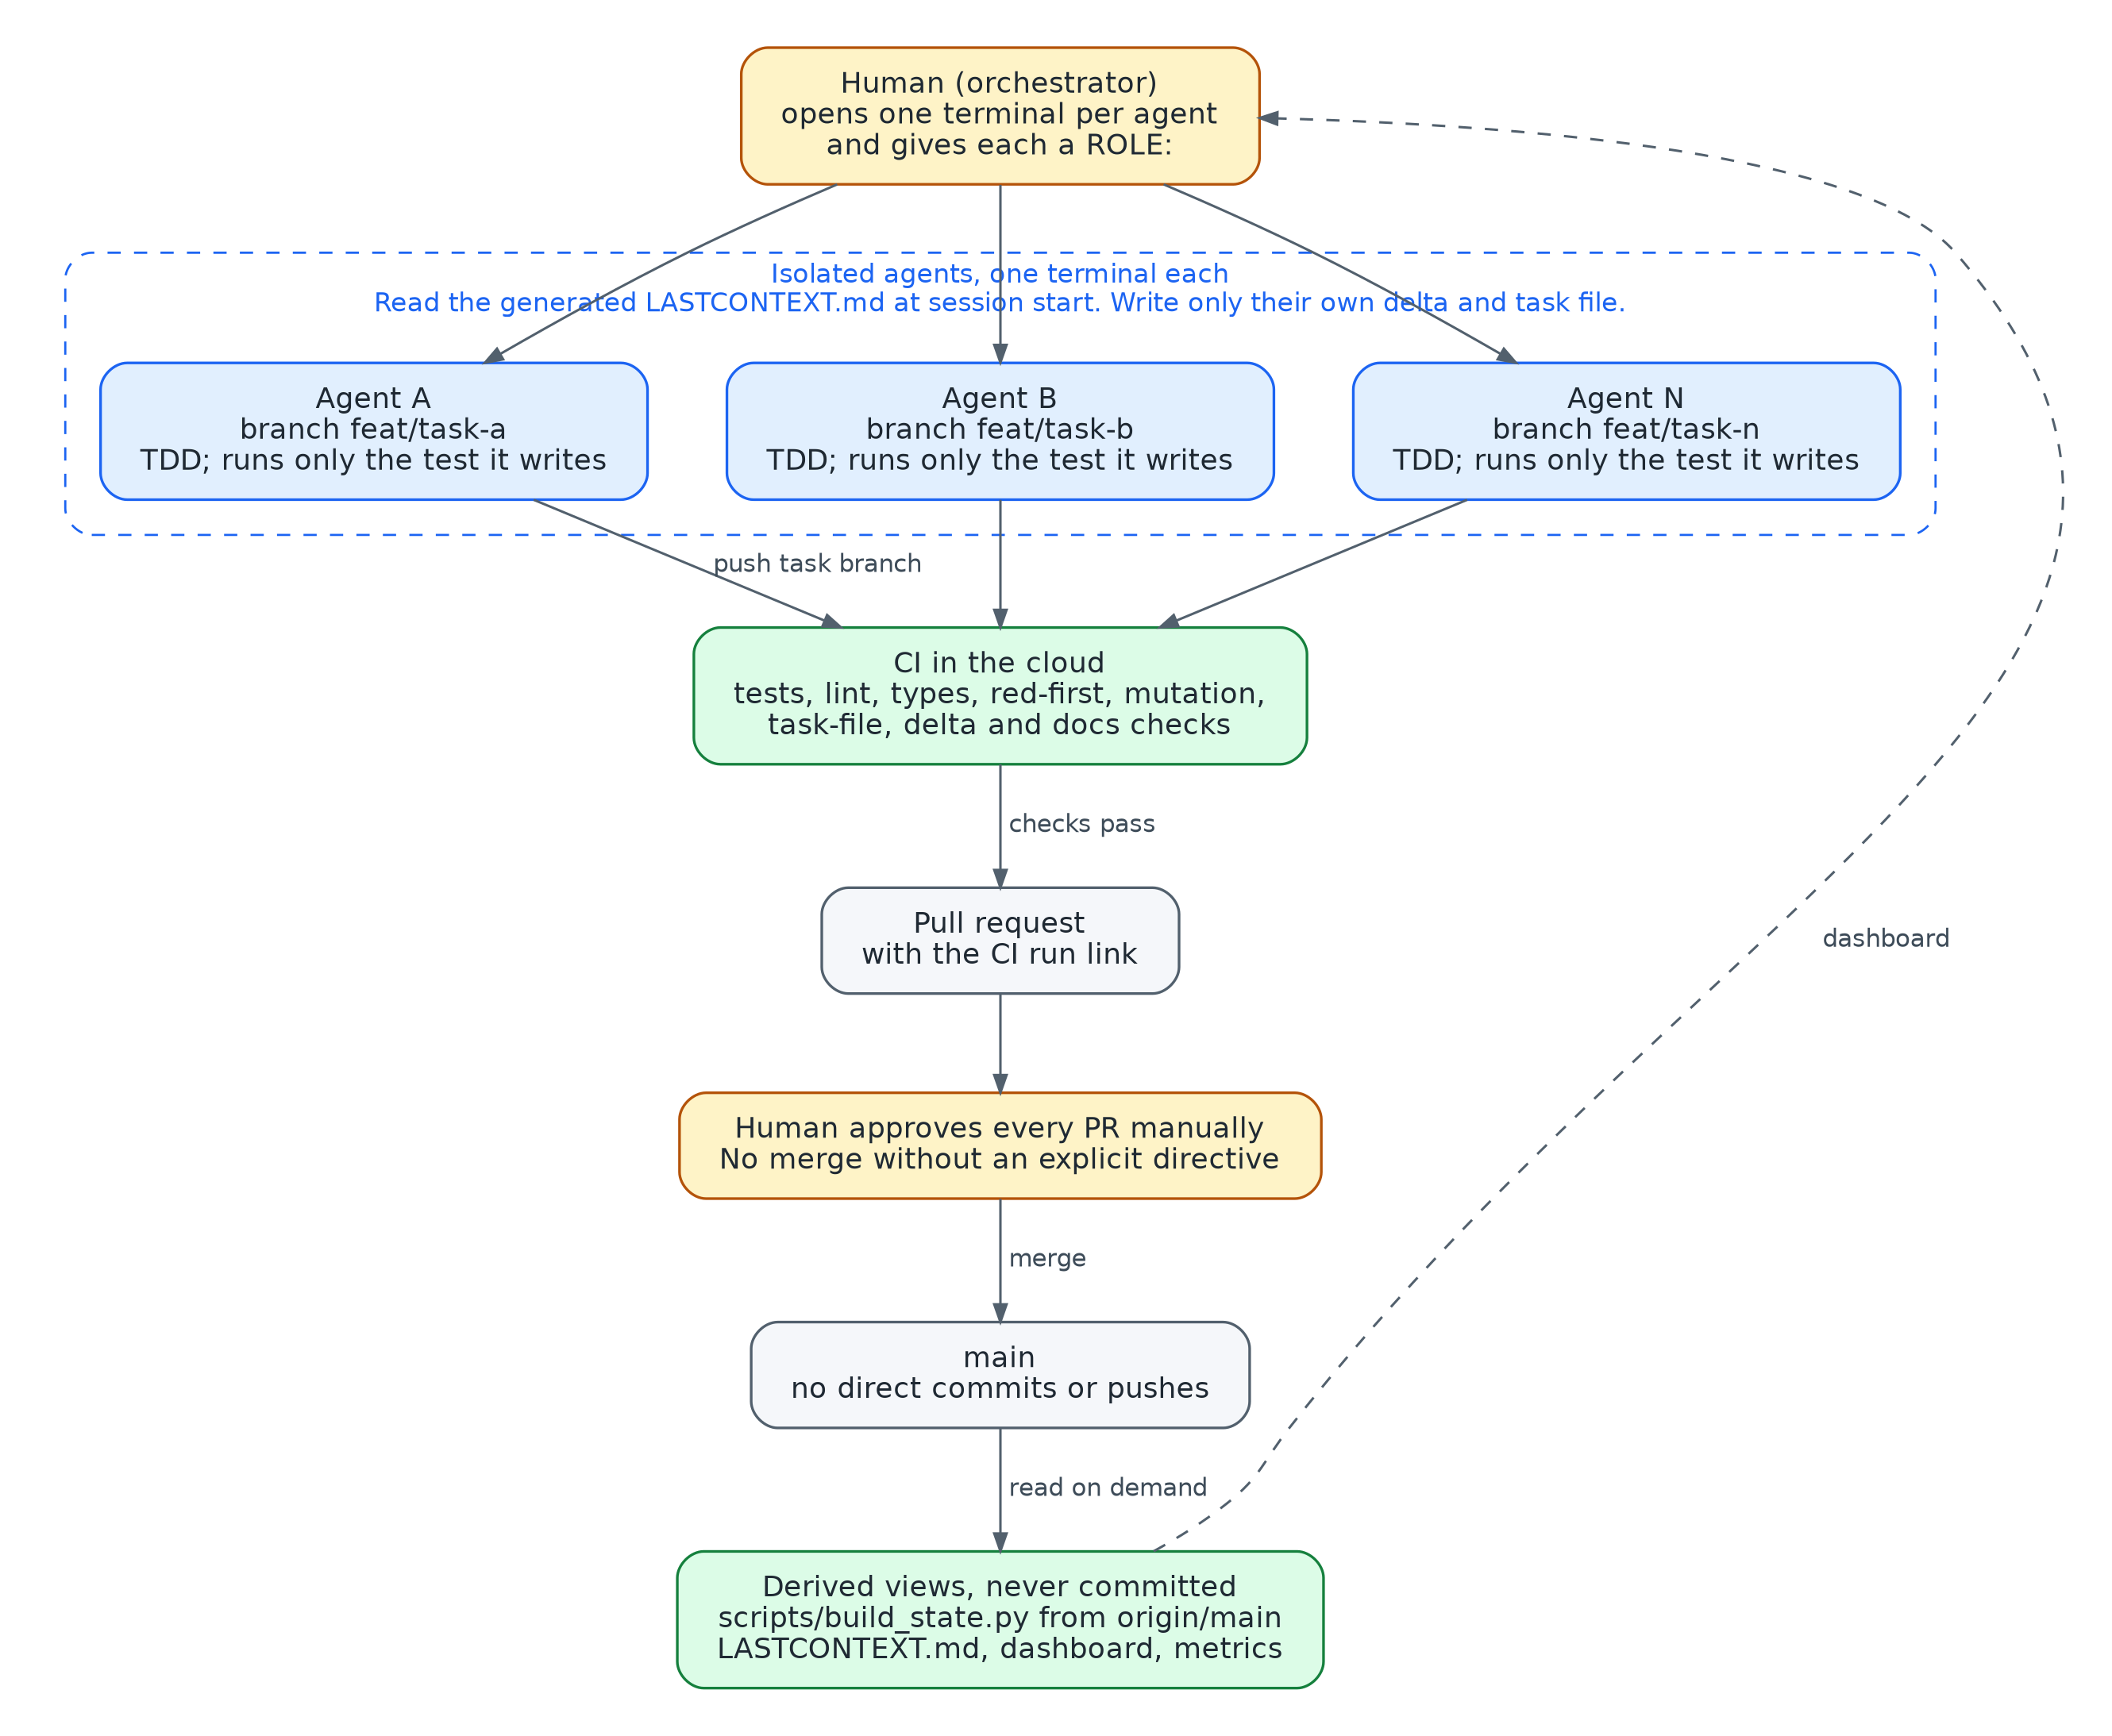
\includegraphics[width=0.8\textwidth,height=0.66\textheight,keepaspectratio]{01-overview.png}
\caption{Overview of AFAW. The three agents are isolated, one terminal each. Blue: agent action; amber: human; green: CI or deterministic check; purple: state files; red: blocked.}
\label{fig:overview}
\end{figure}

\subsection{Roles and session start}

In its first message, the agent asks the human for its role (\code{ROLE:}). A session-start hook builds the shared views from \code{origin/main} with \code{scripts/build_state.py} (Section~\ref{sec:state}) and injects the generated last-context file (Section~\ref{sec:knowledge}) and the roadmap file (\code{PENDING.md}); if the build fails, the agent receives the error instead of a stale copy. The agent also reads the last-context file of its role. Before touching any file it runs \code{git status} and \code{git branch}, because other agents are working in the same repository. It never works on the branch that happens to be checked out: it creates a new, isolated branch first.

\subsection{Task isolation and the life of a task}

Each task gets its own branch, named after the task with a prefix (\code{feat/}, \code{fix/} or \code{chore/}) and a clear description. Work is committed in atomic units: one feature, one commit, in the Conventional Commits format \cite{conventionalcommits}. The agent never commits or pushes to \code{main}. Figure~\ref{fig:lifecycle} gives the twelve steps from the first question to the deletion of the branch.

\begin{figure}[tbp]
\centering
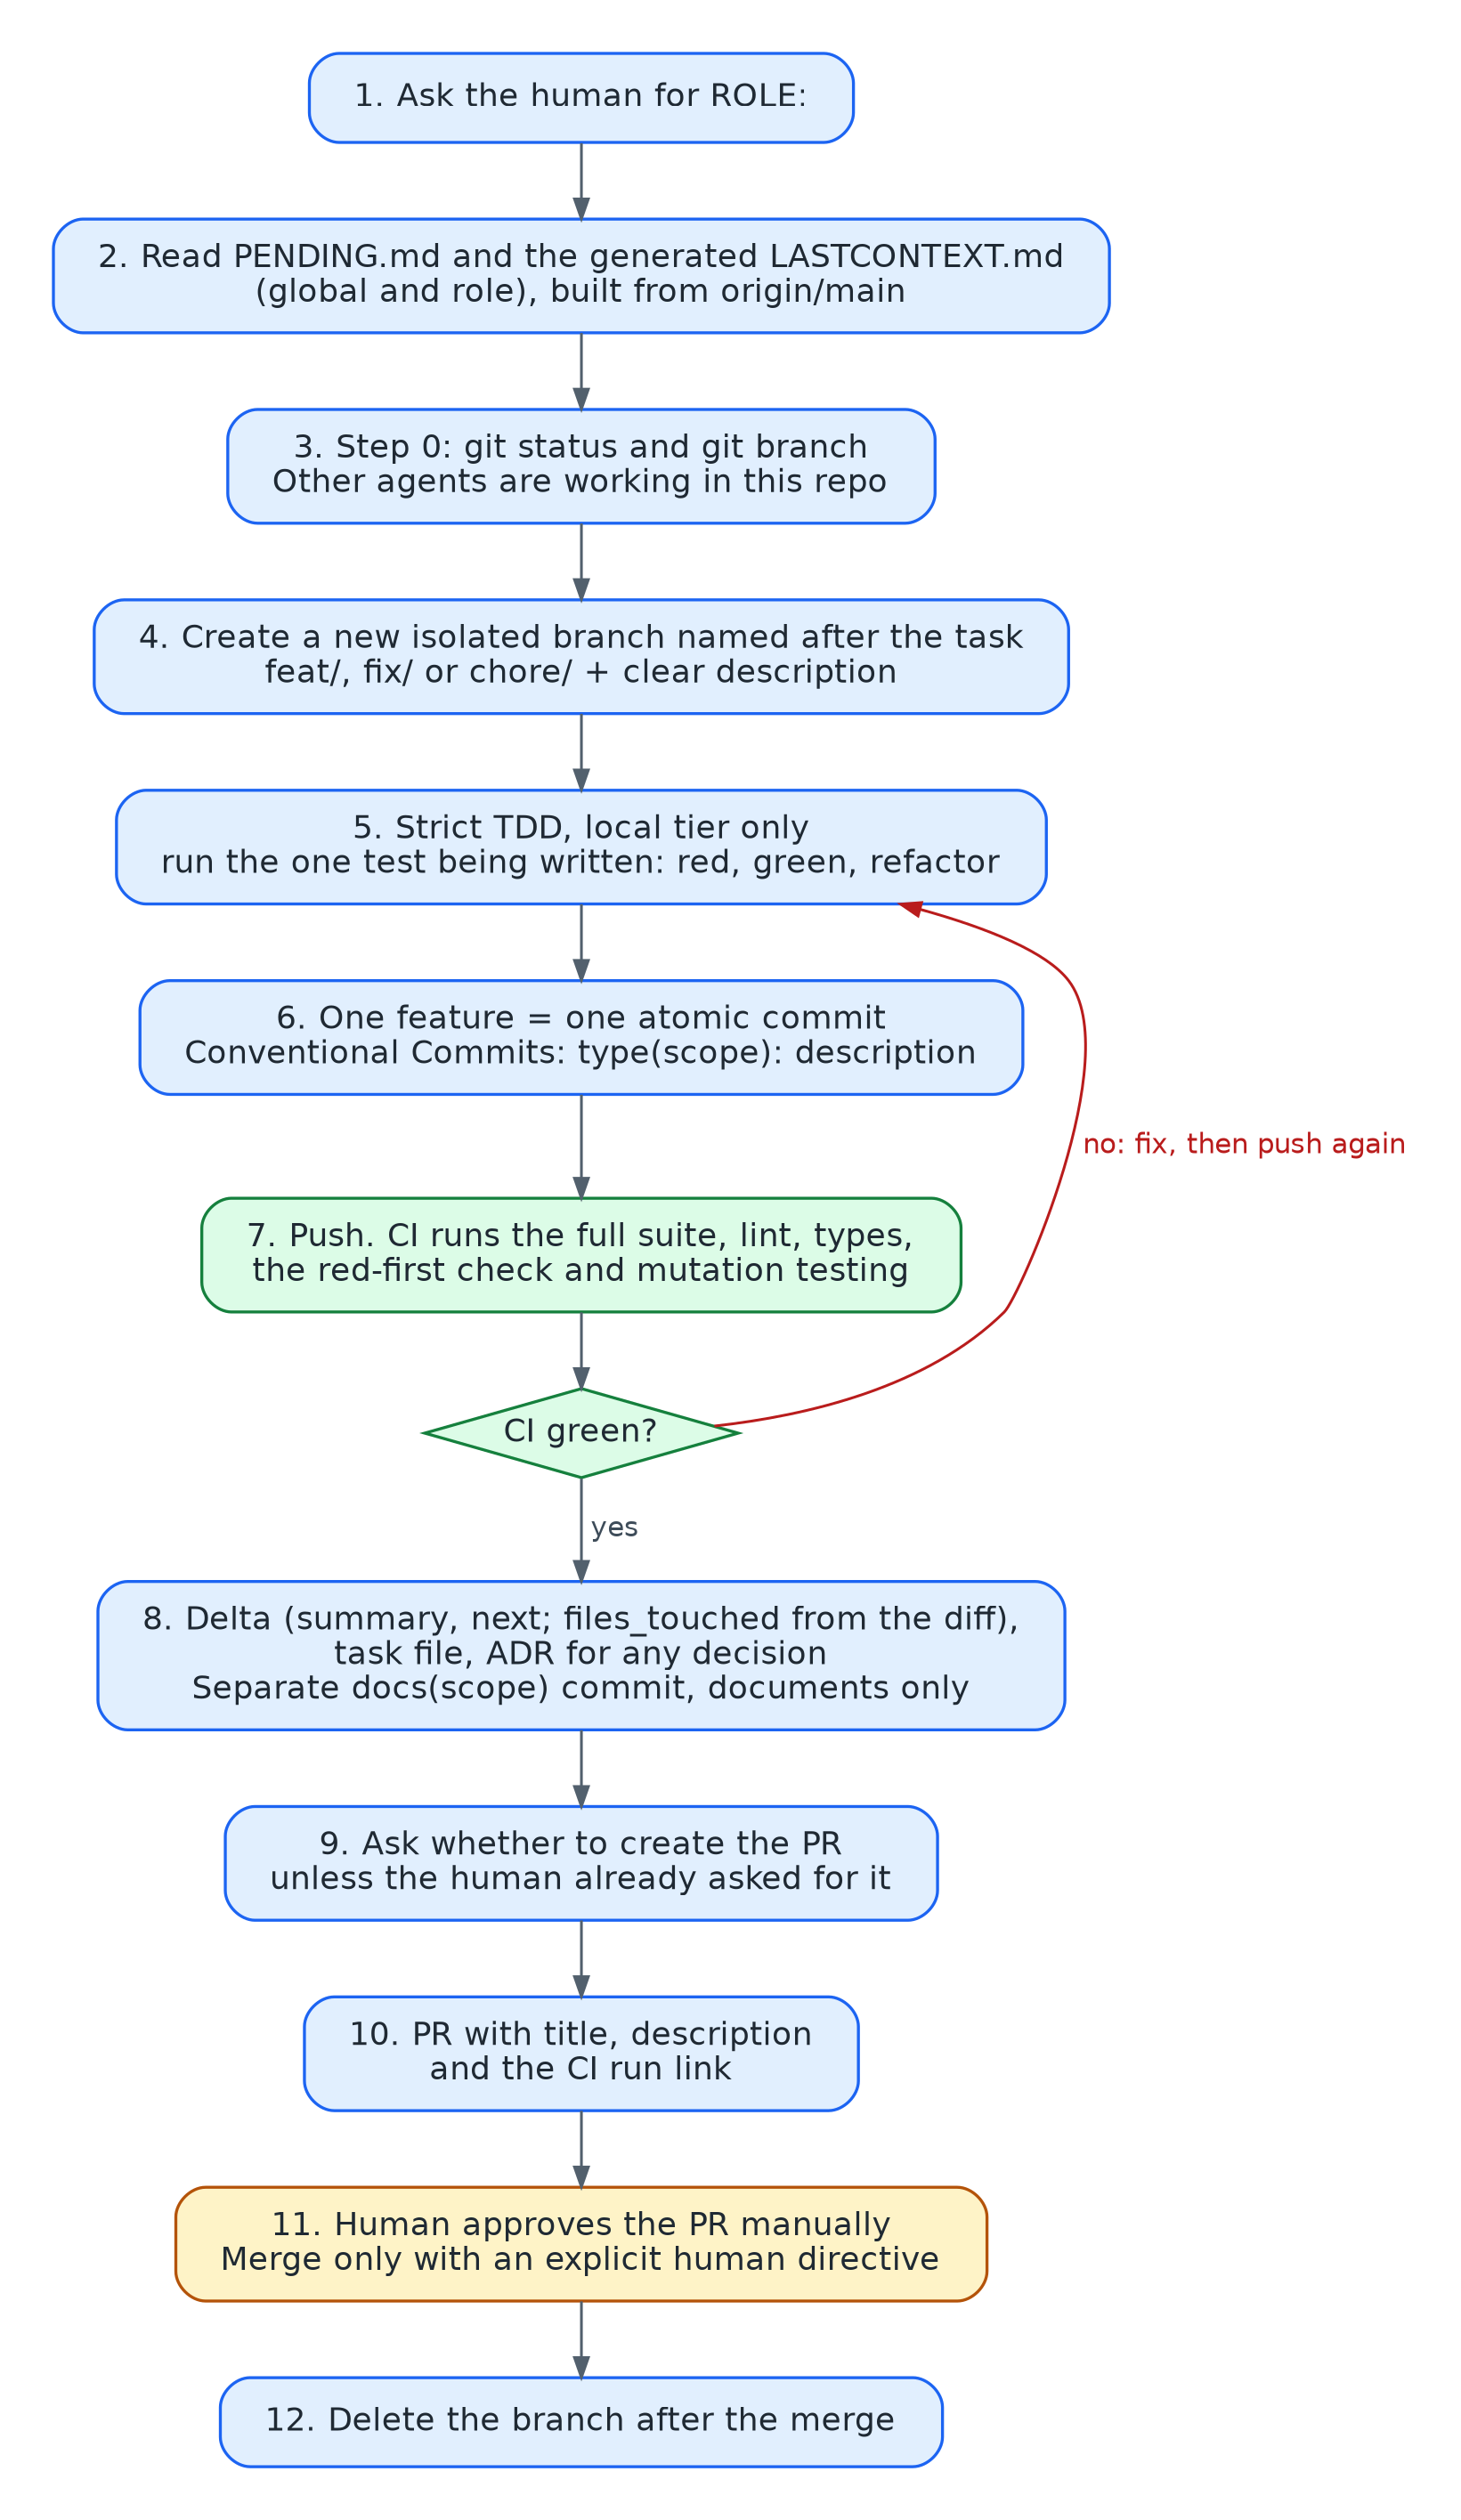
\includegraphics[width=0.64\textwidth,height=0.86\textheight,keepaspectratio]{02-task-lifecycle.png}
\caption{The life of a task, from asking for a role to deleting the branch after the merge.}
\label{fig:lifecycle}
\end{figure}

At the end of a task the agent updates the affected documentation and its own task files, and records them in a separate documentation commit that contains documents only. A decision that constrains later work is recorded as an architecture decision record in the same pull request (Section~\ref{sec:knowledge}). The agent then asks whether to create the pull request, unless the human has already asked for it. The pull request carries a title, a description and the link to the CI run. The human approves it manually, and merging requires an explicit human directive.

\subsection{Isolated state and derived views}
\label{sec:state}

Agents never edit shared state. Each agent writes only two files: its delta (\code{context/tasks/task_NNN_context.json}) and its task file (\code{state/tasks/task_NNN.json}). Because no two tasks write the same file, two pull requests cannot conflict on state. The shared views are derived from these files:
\begin{itemize}
  \item the pending-tasks view (\code{pending.json});
  \item the global last-context file (\code{LASTCONTEXT.md}, Section~\ref{sec:knowledge});
  \item one last-context file per role.
\end{itemize}
They are produced by \code{scripts/build_state.py}, a pure function of the per-task files: the same inputs give byte-identical output (P2). The views are written to a build directory listed in \code{.gitignore}, and CI rejects a pull request that commits one. An agent builds them from \code{origin/main} at session start and whenever it needs a status report. There is no regeneration step after a merge, no bot pull request, and no copy of the state that can go stale on a working branch.

Two consequences follow. First, task identifiers must be unique across parallel branches, so CI rejects a pull request whose task identifier already exists on \code{origin/main}. Second, a view built from \code{origin/main} shows only merged tasks: an agent does not see work in flight on other branches. This is deliberate, because unmerged work has not been approved, but it means that two agents can start overlapping tasks. The roadmap in \code{PENDING.md}, where the human assigns work, is the guard against that.

A CI script (\code{scripts/check_task_delta.py}) checks the delta against the diff. It lists the files changed by the pull request with \code{git diff --name-only} against the merge base, keeps those under the code folders set in \code{state/config.json}, and requires that set to equal the \code{files_touched} field of the delta. A missing or extra entry fails the check. The field is therefore a measured value, not a declaration by the agent. The agent fills it with the same script (\code{--write task_NNN}), so it never writes the list by hand. Figure~\ref{fig:state} shows the flow.

\begin{figure}[tbp]
\centering
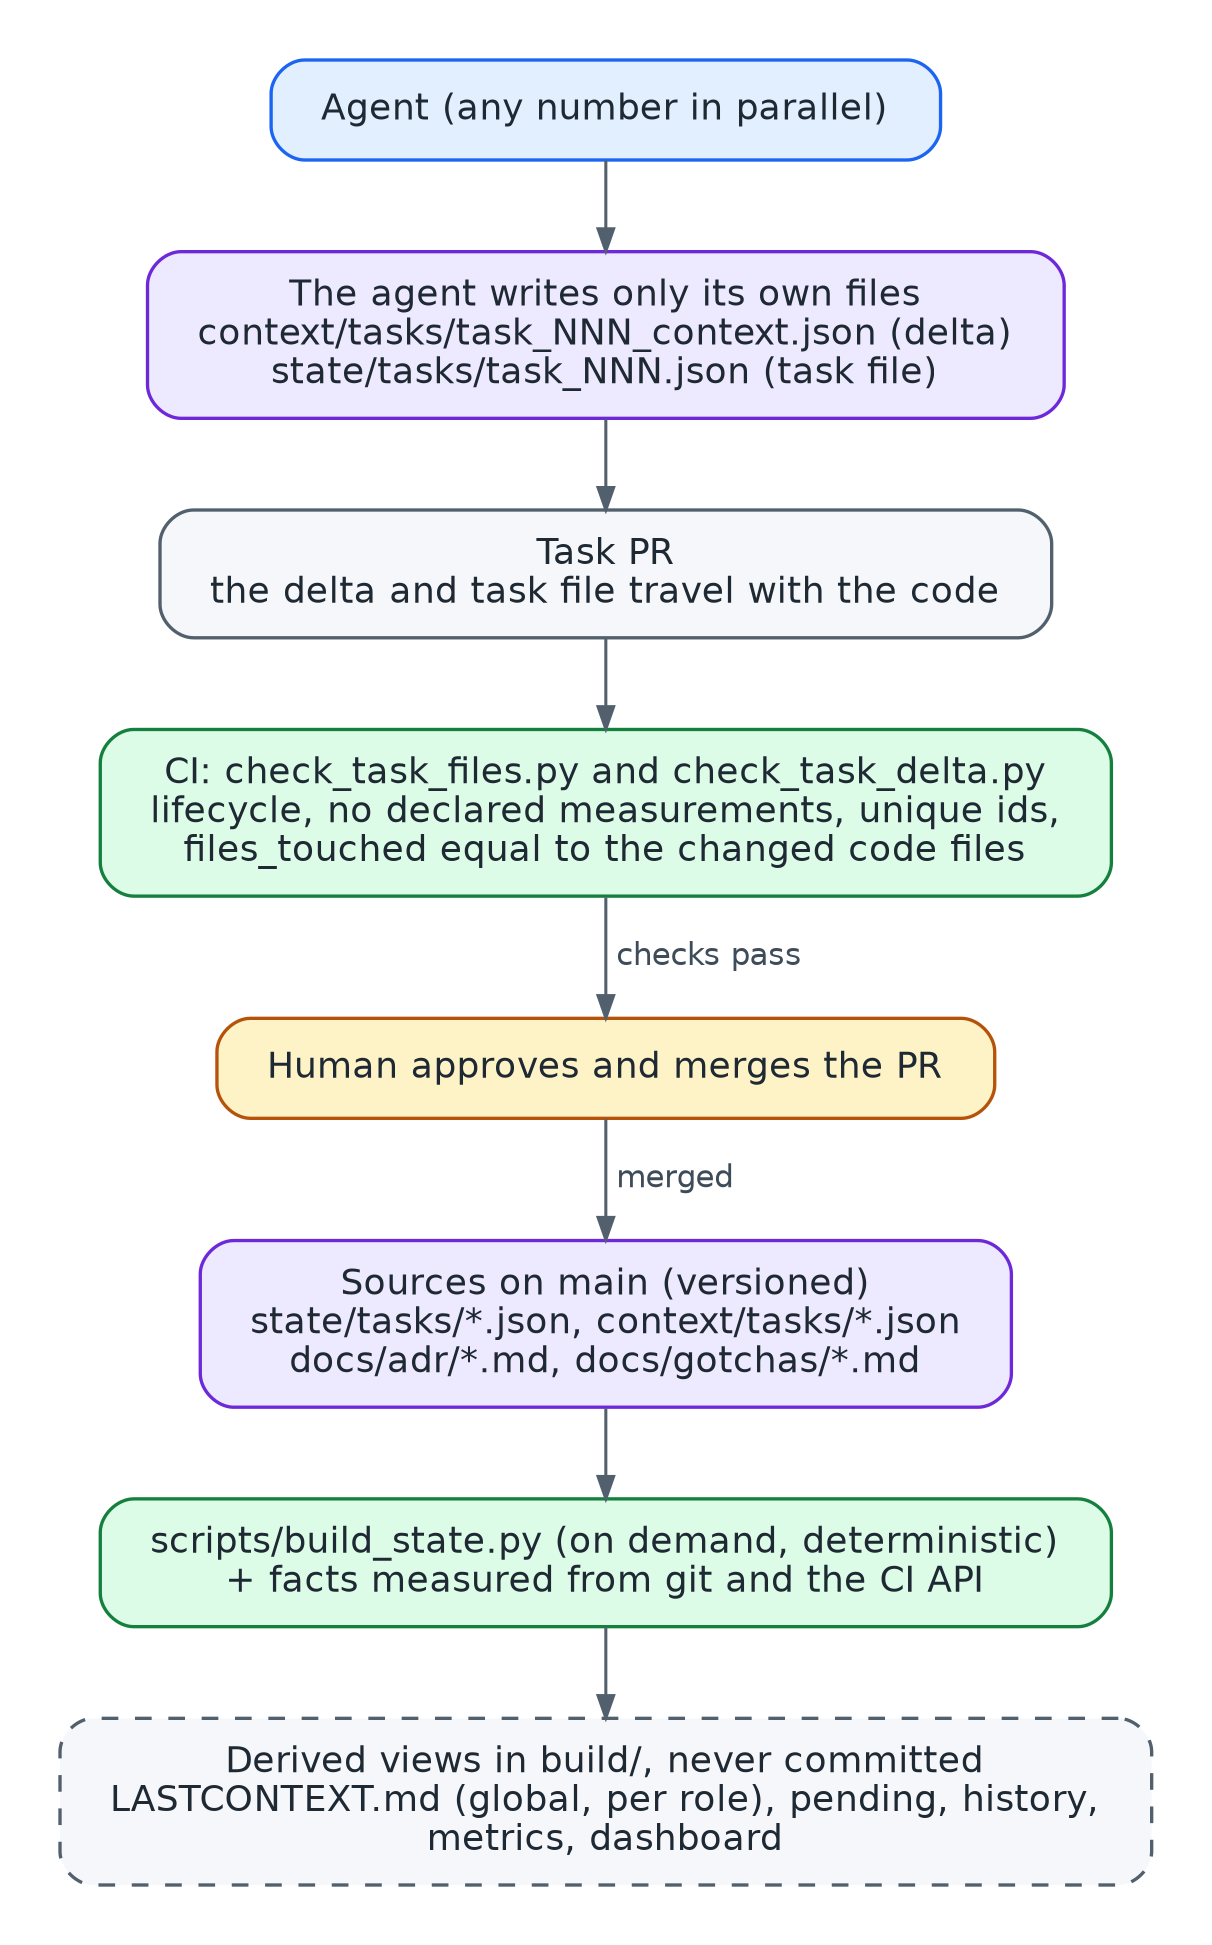
\includegraphics[width=0.5\textwidth,height=0.84\textheight,keepaspectratio]{03-state-and-context.png}
\caption{State and context. The agent writes only its own delta and task file; CI checks the delta against the diff; the shared views are derived from \texttt{origin/main} on demand and never committed.}
\label{fig:state}
\end{figure}

A status report is built from \code{origin/main}, never from a working branch. What it contains, and how each value is obtained, is described next.

\subsection{Task lifecycle, traffic light and timing}
\label{sec:lifecycle}

A task file holds only declared values: identifier, title, role, type, status, priority, difficulty, the tasks it depends on (\code{blocked_by}), its branch and its owner. The owner is an agent by default, or the human for actions only the human can take (approve a pull request, rotate a key, change a repository setting); such a task needs no branch, and a pull request may not change both the owner and the status of a task. The status is one of \code{backlog}, \code{pending}, \code{in_progress}, \code{done} and \code{cancelled}. A pull request sees only its two endpoints: a task that went from pending to in progress to done on its branch arrives as pending to done. So any open status may reach \code{done} in one pull request, a new task may arrive already done, and \code{done} and \code{cancelled} are final. A CI script (\code{scripts/check_task_files.py}) rejects a pull request that reopens a final status, deletes a task file, adds a task identifier that already exists on the target branch, or marks a task in progress or done on a branch other than the pull request's own. Task files are never deleted, so the files of done tasks are the history of the project. A task becomes done on \code{main} only through the merge of the pull request that marked it so.

Measured values are never declared. The same check rejects a task file that contains a timestamp, a CI result or a traffic light. They are collected by \code{scripts/collect_facts.py} from git and from the pull-request and CI interfaces of the hosting platform (Table~\ref{tab:facts}). Pull-request timestamps are used instead of branch commit dates because a squash merge or a rebase rewrites the commits of the branch.

\begin{table}[h]
\centering
\small
\begin{tabularx}{\textwidth}{@{}>{\raggedright\arraybackslash}p{3.9cm}>{\raggedright\arraybackslash}X>{\raggedright\arraybackslash}p{3.3cm}@{}}
\toprule
\textbf{Fact} & \textbf{Definition} & \textbf{Source}\\
\midrule
\code{created_at} & Commit that added the task file to \code{main} & git\\
\code{started_at} & Earliest commit of the task's pull request & Pull-request commits\\
\code{pr_opened_at} & Creation of the pull request & Pull-request API\\
\code{first_green_at} & Earliest time at which every CI run of one commit had finished green & CI API\\
\code{merged_at} & Merge of the pull request & Pull-request API\\
\code{last_activity_at} & Latest commit or CI run on the branch & git, CI API\\
CI status & State of the runs of the latest commit: success, failure or pending & CI API\\
CI usage & Runs, failed runs, jobs, queue time, job minutes & CI API\\
\bottomrule
\end{tabularx}
\caption{Measured facts per task. None of them is written by an agent.}
\label{tab:facts}
\end{table}

\textbf{Traffic light.} The light is a rule, not an assessment by the agent (P1). The conditions are checked in this order:
\begin{itemize}
  \item \emph{red}: a task it depends on is not done, or CI fails on the latest commit of its branch;
  \item \emph{no data}: a task in progress for which no fact was measured, shown as such rather than as green (P6);
  \item \emph{yellow}: a task in progress with no commit and no CI run for more than a set number of days (\code{stale_days} in \code{state/config.json});
  \item \emph{green}: every other open task.
\end{itemize}
Backlog, done and cancelled tasks have no light. The priority is set by the human. The difficulty is a declared estimate and is labelled as such in every view.

\textbf{Durations.} Three wall-clock durations are derived for each task, and kept apart because they measure different things:
\begin{itemize}
  \item \emph{agent time}, from \code{started_at} to \code{first_green_at}: work until CI first passes;
  \item \emph{review latency}, from \code{pr_opened_at} to \code{merged_at}: the human's time, not the agent's;
  \item \emph{lead time}, from \code{started_at} to \code{merged_at}: the total.
\end{itemize}

\textbf{CI usage.} For each task, the number of runs and of failed runs, the queue time (the sum over jobs of the start time minus the creation time) and the job minutes (the sum over jobs of the duration rounded up to a whole minute, the unit in which GitHub bills standard runners). Price multipliers for other runner types are not applied; the platform's billing report remains the ground truth for cost.

\textbf{Views and dashboard.} \code{scripts/build_state.py} derives the pending view, a history of done tasks ordered by merge time, the last-context views, a metrics file and a static HTML dashboard. Aggregates are the median and the quartiles over done tasks, with the number of tasks for which a value is missing; a missing value is counted, never filled in. Progress is the number of done tasks over the number of tasks not cancelled. It is a count: every task weighs the same, because the only size available, the difficulty, is an estimate. The dashboard also shows the tasks by status and the tasks merged per day, as charts drawn when the page is built.

The reference time is an explicit input: by default the commit time of the ref being read, never the clock, so the same ref, facts and reference time give byte-identical views (P2). The dashboard is rebuilt on every push to \code{main}, and also on a schedule: the light of a task in progress depends on the CI and the activity of its branch, which change without any commit to \code{main}. A scheduled run passes its own time as the reference, so inactivity is measured against the run. The dashboard contains no scripts and loads nothing when viewed. It can be opened locally, kept as a CI artifact, or published as a static site; a public site exposes the backlog.

\subsection{Project knowledge and the last-context file}
\label{sec:knowledge}

State files say \emph{what} is happening; they cannot say \emph{why}. A decision recorded as one line of data does not say which problem it solves or which alternatives were rejected, and a later agent or person who does not know the reason is likely to reverse it. Recording the same knowledge twice, once as data and once as prose, creates a second problem: the two copies drift apart. AFAW therefore keeps one source per kind of knowledge, and the source of knowledge is prose.

\begin{itemize}
  \item \textbf{Decisions} are architecture decision records \cite{nygard2011} in \code{docs/adr/NNNN-slug.md}, with the sections Context, Decision, Alternatives considered and Consequences. Rule: a decision that constrains later work is recorded as an ADR in the pull request that introduces it, and the human accepts it there.
  \item \textbf{Gotchas}, operational traps that still apply, are short records in \code{docs/gotchas/NNNN-slug.md}, with the sections Symptom and What to do.
  \item \textbf{Architecture and environment} descriptions are ordinary documents, written and updated by hand.
  \item \textbf{What was done and what was not} in a task is in its pull request and in the \code{summary} and \code{next} fields of its delta.
\end{itemize}

Each record starts with a small front-matter block that holds only what a program needs: status, date, tags and links to other records (\code{supersedes} for an ADR; \code{resolved_by} or \code{promoted_to} for a gotcha). A CI script (\code{scripts/check_docs.py}) checks file names, front matter, required sections, the consistency of the \code{supersedes} chain, and that relative links in the documentation resolve. It cannot tell whether a decision that should have been recorded is missing; that remains the reviewer's judgement.

The global last-context file, \code{LASTCONTEXT.md}, is generated by \code{scripts/build_state.py} and never written by hand. Its sections follow the questions an agent asks at the start of a session: where things stand (progress, and each task in progress with its light and the summary and next steps of its delta); what is waiting on the human; the next tasks in order; the decisions in force and those proposed; the active gotchas; and the reference documents to read. Decisions and gotchas appear as one line each, with the path to the record, so the file is an index to documents rather than a copy of them. A per-role file shows the same index filtered by tags configured for the role, together with the tasks most recently merged in that role.

Nothing in the file grows by accumulation. The parts about tasks are bounded by the open tasks. A record leaves the index only for an explicit reason, never because of its age: an ADR is superseded or deprecated; a gotcha is resolved, with the task that fixed its cause, or \emph{promoted}, with the mechanism that now enforces it (a hook, a script, a configuration default or a test). Promotion is the preferred exit, because a rule enforced by a mechanism no longer depends on the agent reading it (P7). As a last control, the number of active records is measured against a configured budget; above it, the dashboard reports that a review is due, and the human prunes in a pull request. No record is deleted or summarized automatically: deciding that knowledge no longer applies is a judgement, and a generated summary would be an unmeasured claim (P1).

\subsection{Verification: local and CI tiers}
\label{sec:ci}

Development is test-driven in the strict sense: the agent writes a test, confirms that it fails, writes the minimum code that makes it pass, and refactors with the test green. For a bug, the first step is a test that reproduces it and fails. When the task is to add tests to existing code, only the test folder is edited. If a new test fails against the original code, the test is presumed wrong unless there is evidence of a real defect, in which case it is marked as an expected failure with the reason recorded, and the source is not changed to make it pass.

The red--green loop needs a test run at every step, and a push to CI per step would be too slow to follow. Execution therefore has two tiers. On the local machine, the agent runs only the tests it is writing, one test or one test file at a time. This tier must finish within seconds and must not need external services. Everything else runs in CI.

A red step seen locally is still a claim by the agent (F3). CI turns it into a measurement with a red-first check (\code{scripts/red_check.py}). The check takes the test functions added by the pull request, runs them against the code at the merge base, and requires each of them to fail. A new test that passes on the old code did not drive the change, and the check fails. Some tasks add tests that are meant to pass on the old code: tests for existing code, and refactors with no change in behavior. Their task file declares the type (\code{tests-only} or \code{refactor}); the check is then skipped, and the declaration is shown to the reviewer. Within a feature, a single test that documents behavior the code already has is declared with a \code{characterization} marker and a reason, and is printed in the same way. A test that does not appear in the report of the old run did not run, and the check fails rather than count it as passing. On the pull request that introduced these scripts, the check rejected four tests; one of them passed on the old code for the wrong reason (it asserted only a non-zero exit, which a missing module also gives) and was rewritten.

The full test suite, linters, type checks, mutation testing and builds run in CI. Independent jobs run in parallel, and path filters make each job run only when its own files change: back-end changes launch back-end jobs, front-end changes launch front-end jobs, and document-only changes launch nothing. Linters run only on the modified files. Load and chaos tests run as manual or scheduled workflows, not on every pull request. Figure~\ref{fig:ci} summarizes the pipeline.

\begin{figure}[tbp]
\centering
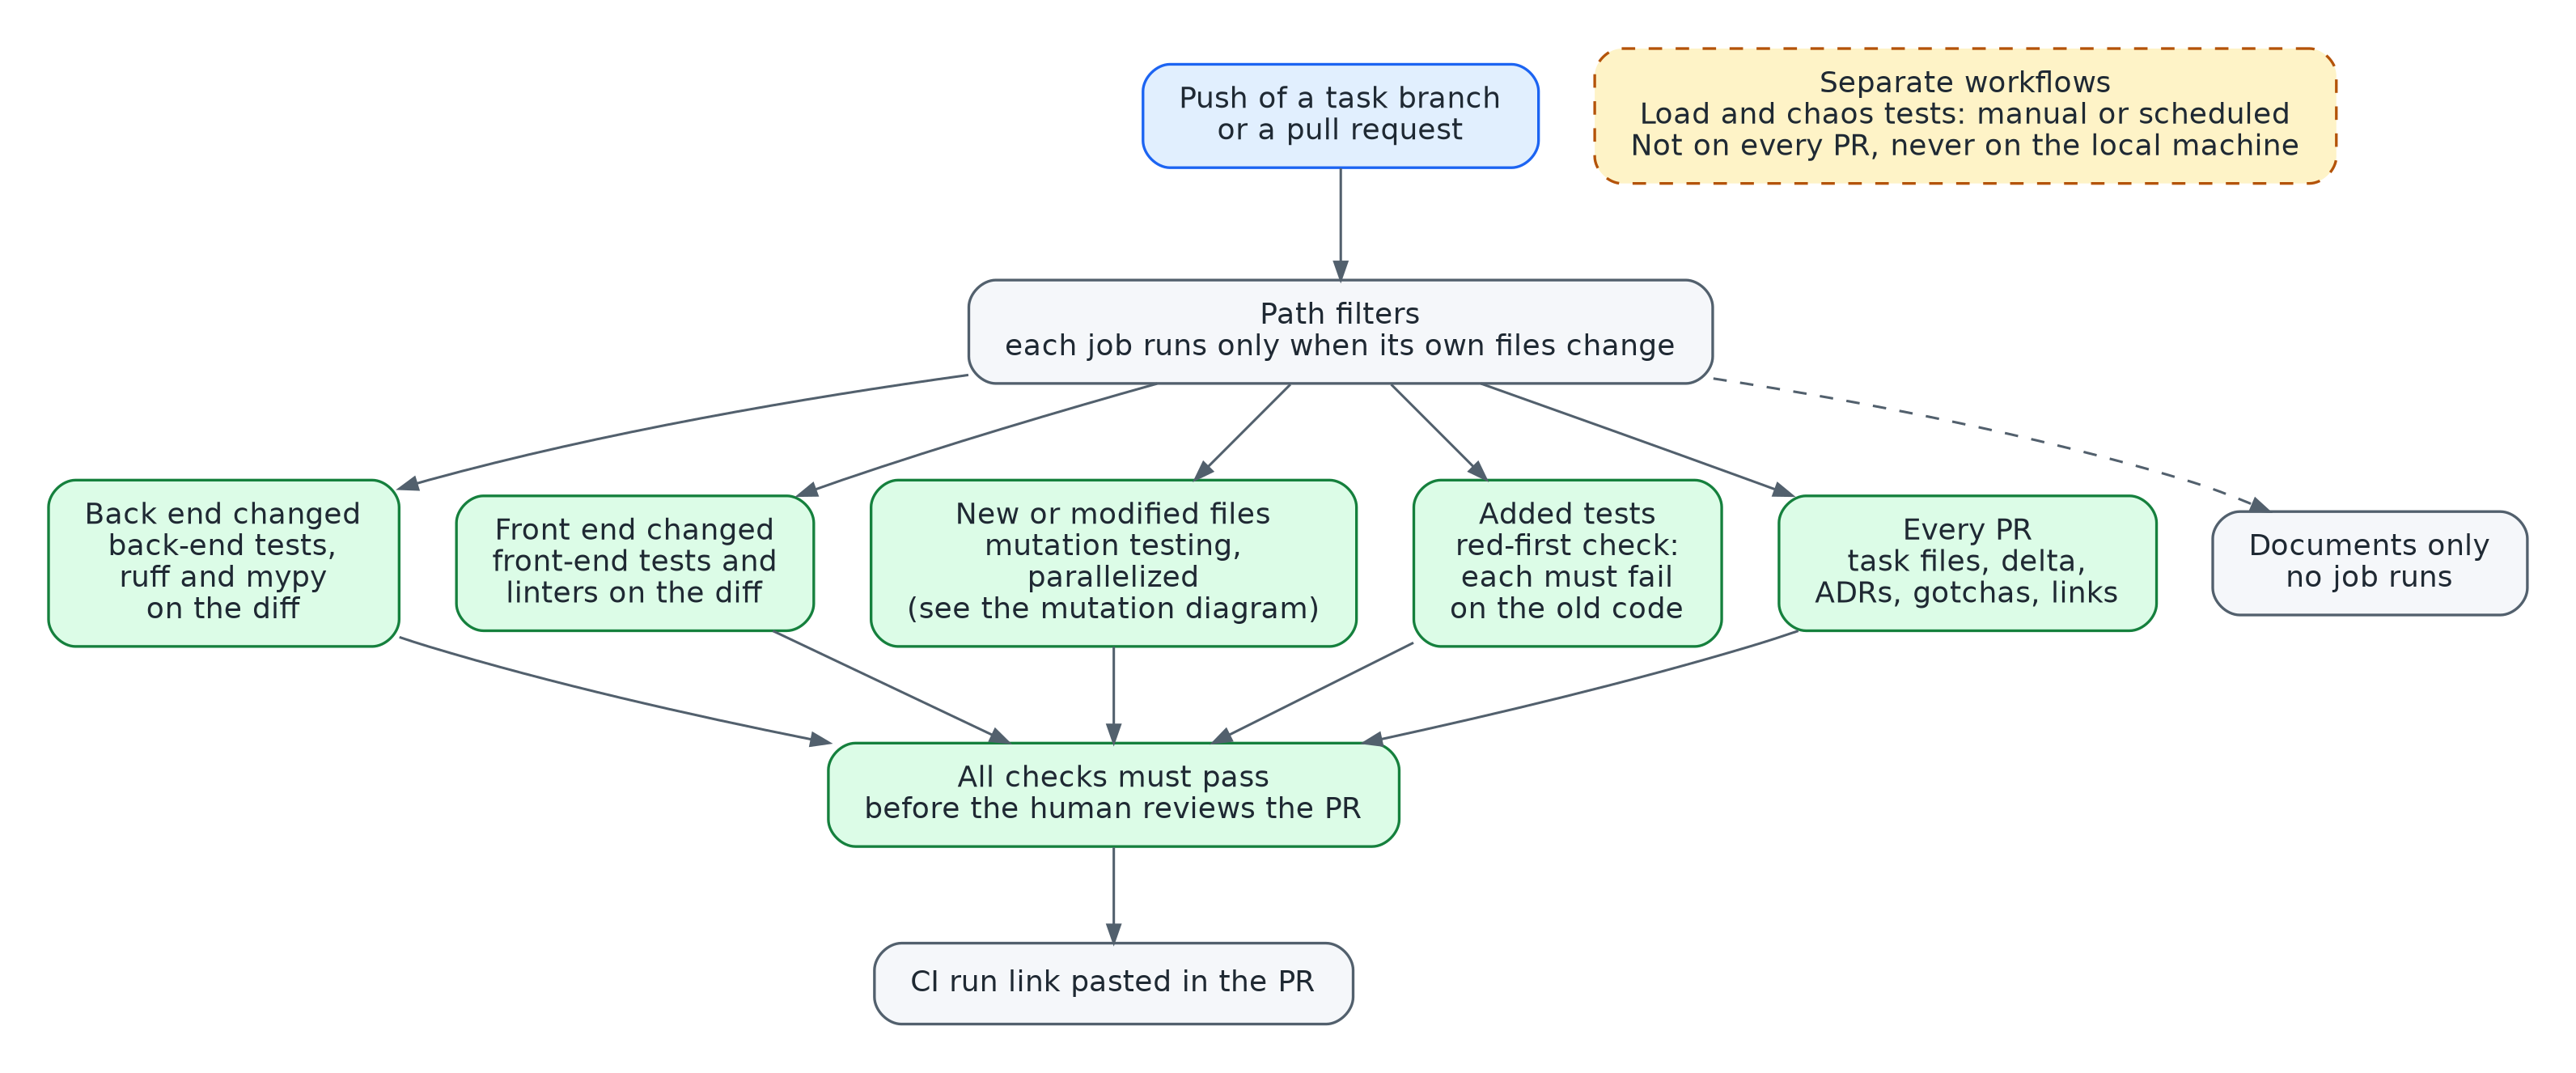
\includegraphics[width=0.92\textwidth,height=0.42\textheight,keepaspectratio]{04-ci-pipeline.png}
\caption{The CI pipeline. Path filters route a change to parallel jobs, including the red-first check; load and chaos tests are separate workflows.}
\label{fig:ci}
\end{figure}

Verification rules apply to the checks themselves. A script that reports PASS does not prove that it measured the right thing, so internal consistency (two runs agree) is combined with a known external value. Credentials and configuration are validated before minutes of compute are spent.

\subsection{Mutation testing on the diff}
\label{sec:mutation}

Mutation testing \cite{demillo1978,jia2011} alters the source in small ways (mutants) and re-runs the tests. If the tests still pass, no test detected that change. The line may well be executed; no assertion depends on it. With $N$ generated mutants, $K$ killed and $E$ equivalent to the original, the mutation score is $K/(N-E)$. Coverage and mutation score measure different things and should be reported separately.

AFAW applies mutation testing only to new or modified files, in parallel in CI (Figure~\ref{fig:mutation}). Before mutating, the baseline is validated: the suite must pass on unmodified code, otherwise every mutant would count as killed and a false 100\% would result. Surviving mutants are fixed by writing or improving tests, and the run is repeated. A survivor believed to be equivalent follows the procedure below; it is never covered with an artificial test. The step is mandatory in critical modules (money, security, concurrency, public contracts), where a file below the minimum score blocks the pull request. The critical paths and the minimum score are defined per project in \code{state/config.json} (\code{mutation_critical_paths} and \code{mutation_min_score}).

The denominator is where the gate can be gamed. Whether a mutant is equivalent is undecidable in general, and an agent that marks survivors as equivalent lowers $N-E$ until the gate passes: an unmeasured claim again (F3). AFAW therefore separates the proposal from the decision. The agent may propose a survivor as equivalent, with a justification, in the pull request. Only the human records an accepted equivalence, in \code{state/equivalent_mutants.json}. A hook denies agent writes to that file, and CI lists every change to it in the pull request summary. Each entry names the file, the mutant and a hash of the file content, so the entry expires when the file changes. The gate uses $K/(N-E_h)$, where $E_h$ counts only equivalences accepted by the human. The raw score $K/N$ is reported next to it, and expired equivalences are listed rather than counted. The mutation engine stays project-specific; \code{scripts/mutation_gate.py} applies the gate to its results.

\begin{figure}[tbp]
\centering
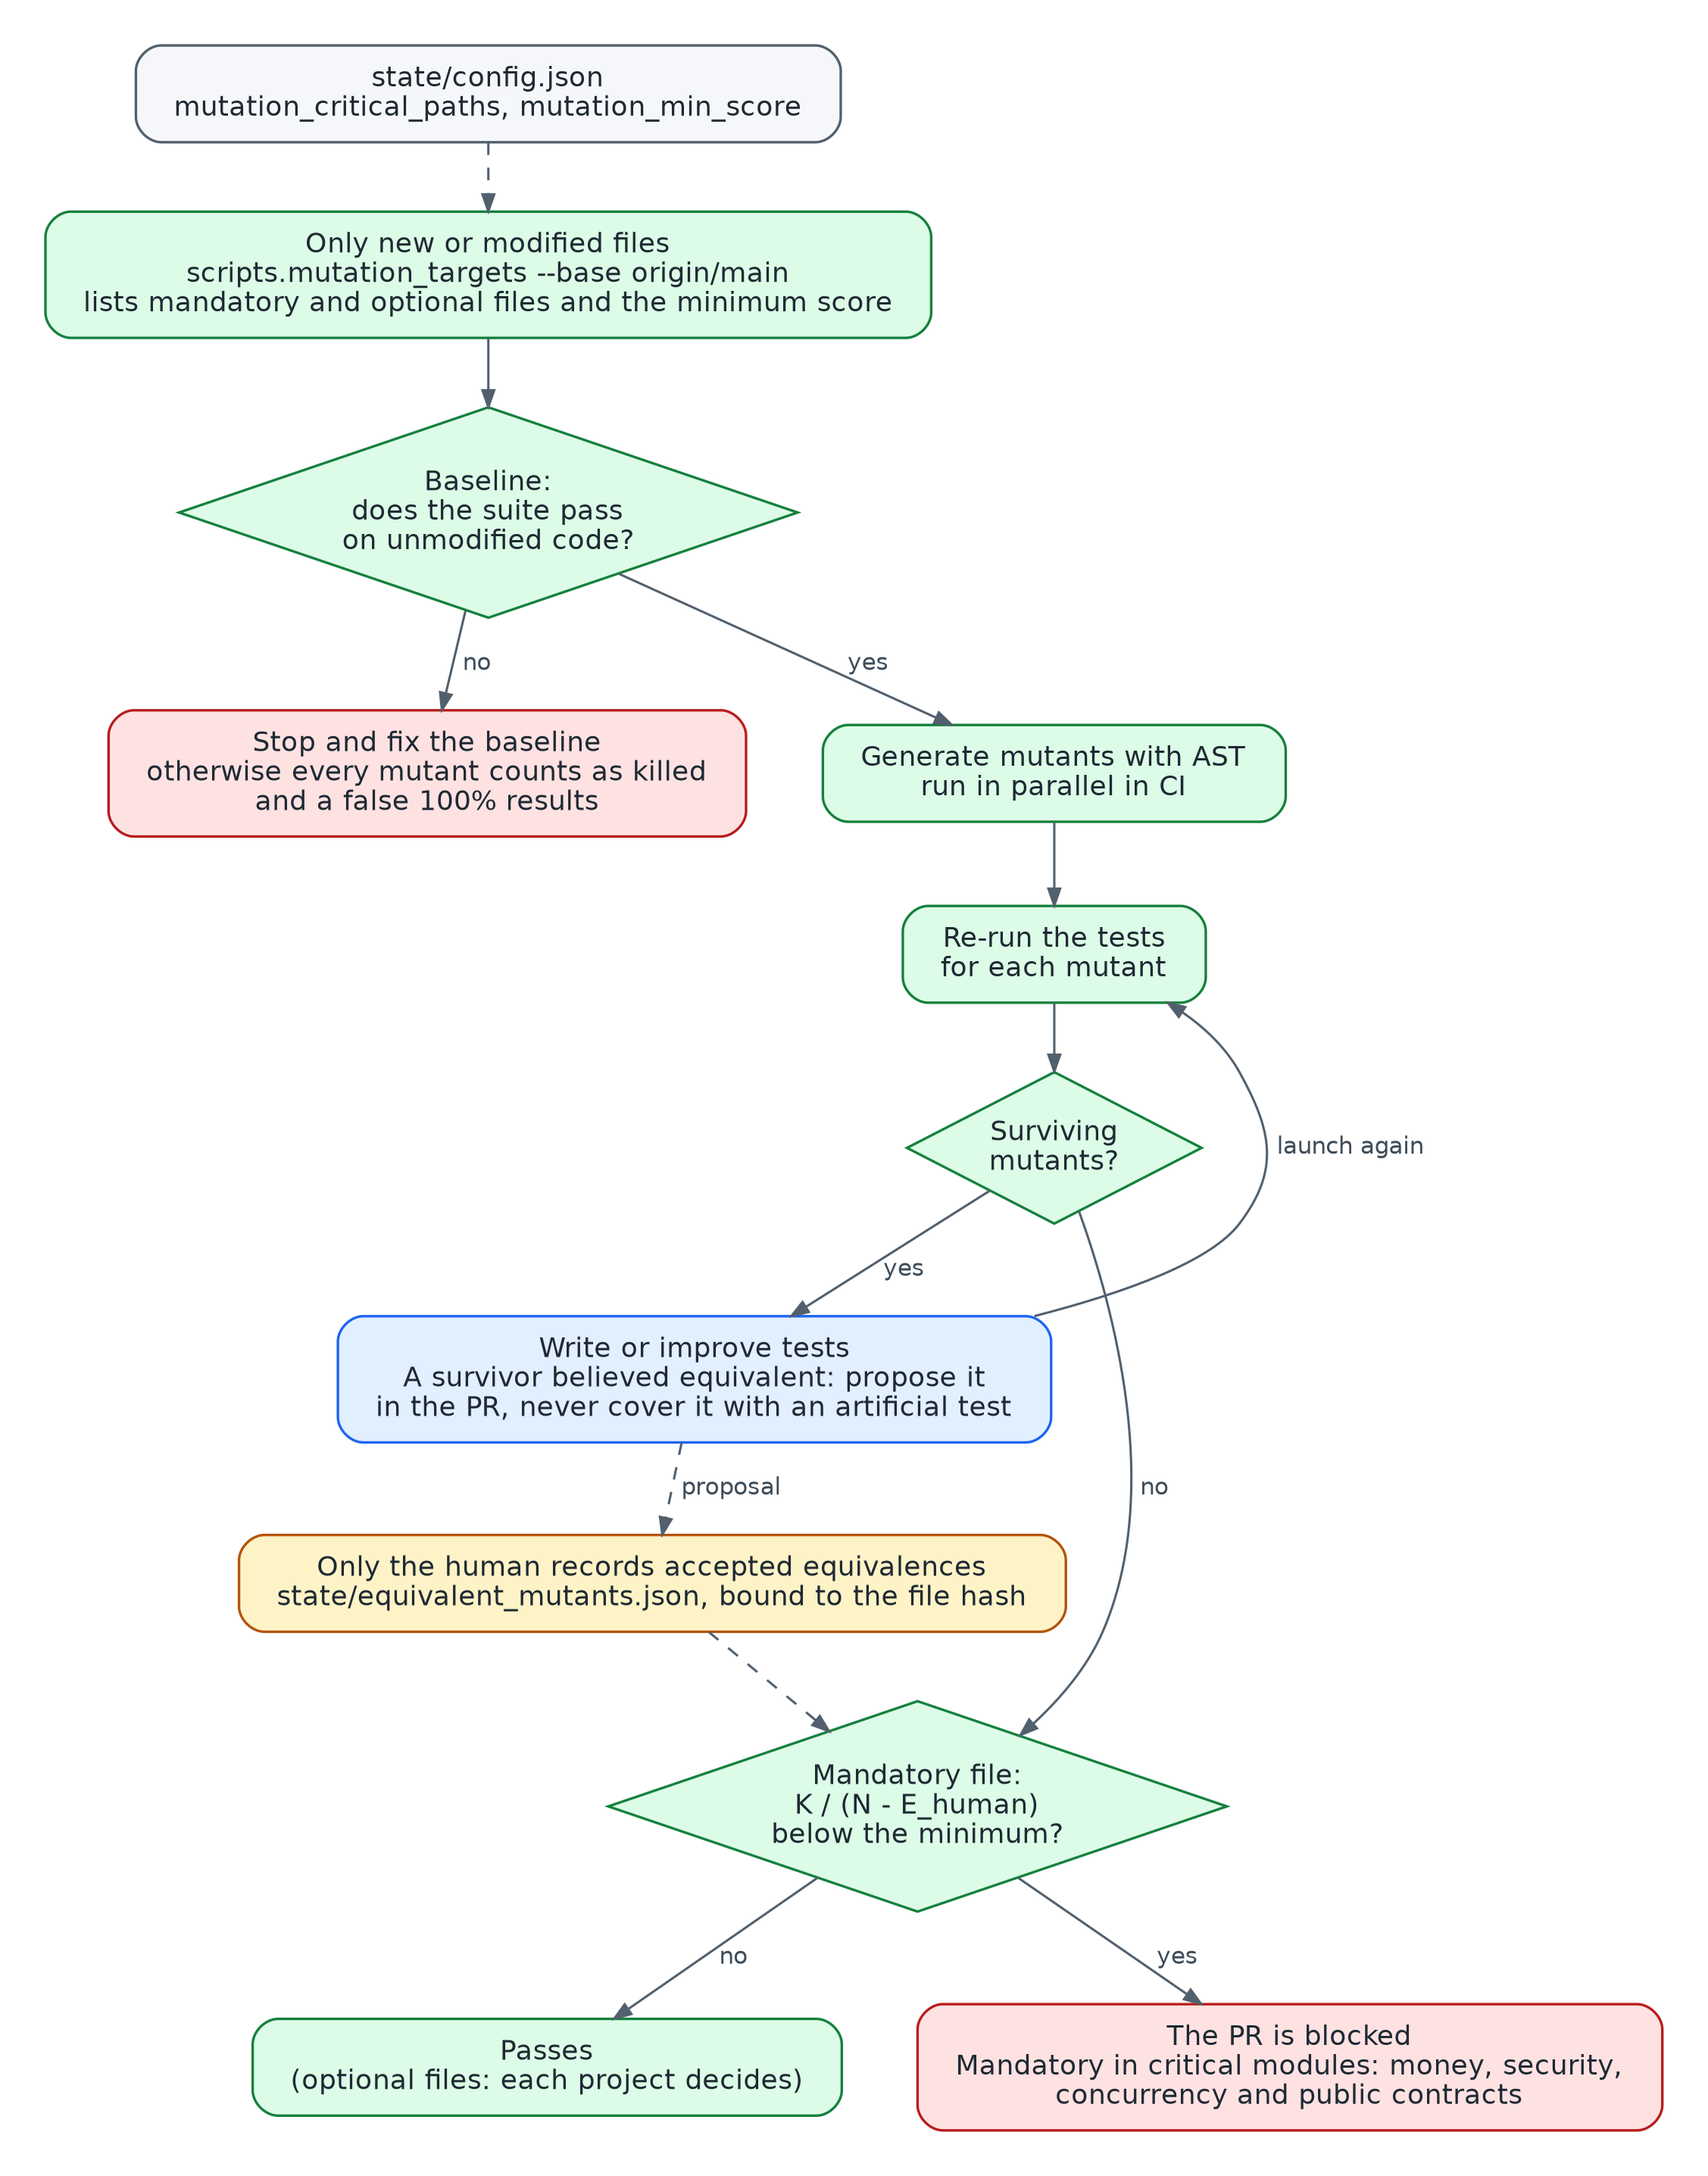
\includegraphics[width=0.94\textwidth,height=0.74\textheight,keepaspectratio]{05-mutation-testing.png}
\caption{Mutation testing on the diff, with the baseline check, human-only acceptance of equivalent mutants, and the blocking rule for mandatory files.}
\label{fig:mutation}
\end{figure}

\subsection{Human authority and enforcement layers}
\label{sec:enforcement}

The rules ``never commit or push to \code{main}'', ``never merge without an explicit human directive'' and ``the human approves every pull request'' are written in the agent instruction file. Because that file is advice (P7), they are also placed under mechanisms that do not depend on the model (Figure~\ref{fig:layers}). Hooks intercept commands before they run. Hard-deny rules let \code{PENDING.md} be edited but never deleted or emptied, deny agent writes to \code{state/equivalent_mutants.json} and to the generated files under \code{build/}, and deny a push to \code{main}. CI checks block a pull request that fails tests, lint, types, mutation, the red-first check, the task-delta check or the task-file check. Branch protection on \code{main} makes the server reject a direct push. The human approval is the last step.

\begin{figure}[tbp]
\centering
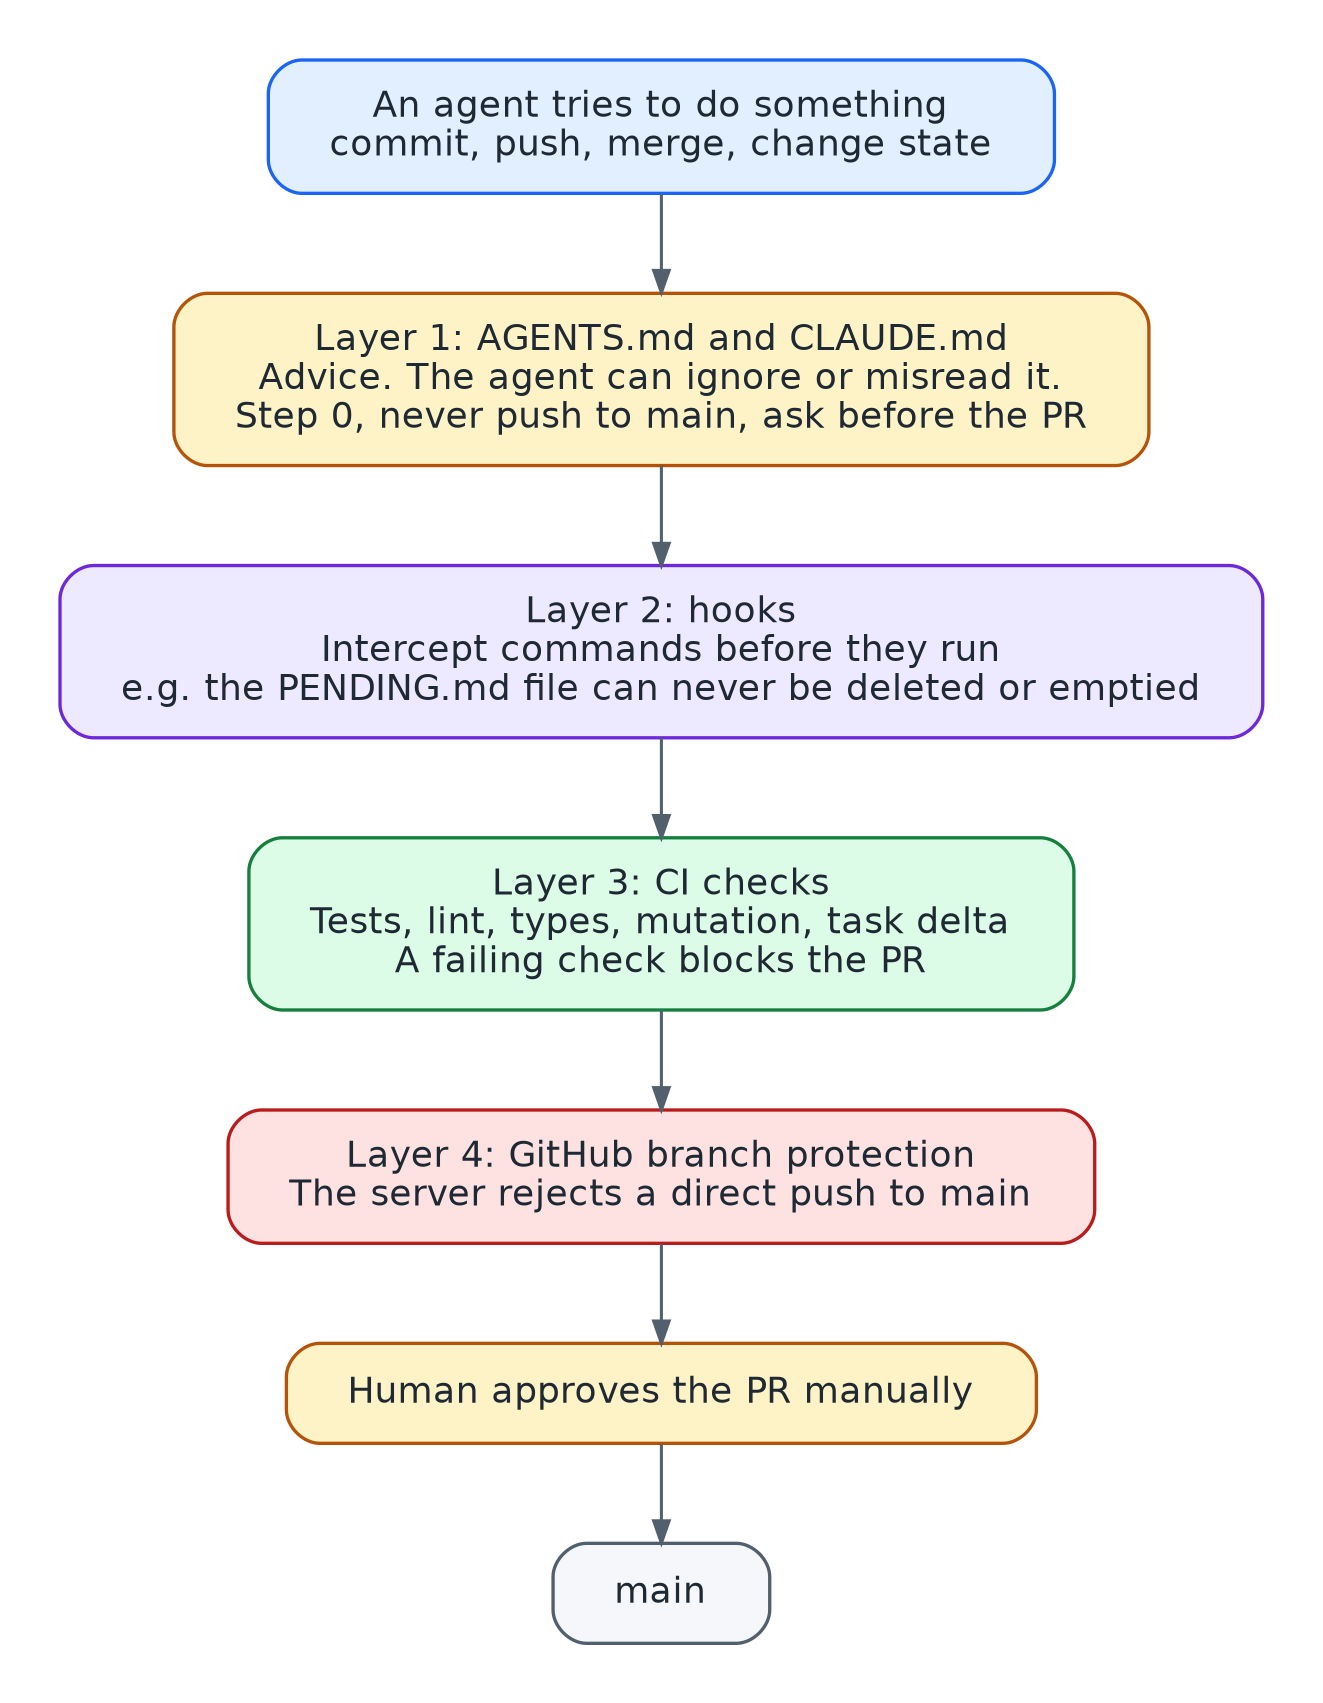
\includegraphics[width=0.56\textwidth,height=0.55\textheight,keepaspectratio]{06-control-layers.png}
\caption{Control layers. The layers are shown in a rough order; in practice each acts at a different moment.}
\label{fig:layers}
\end{figure}

Hooks are a best-effort filter, not a security boundary: a command can be phrased in a way a pattern misses. Branch protection is the barrier that does not depend on the agent.

\subsection{A module for systems that embed an LLM}

When the product itself contains LLM agents (F7), AFAW adds rules that follow the same principles. The LLM never executes tools with side effects: only deterministic code does, and every write tool is idempotent by a request identifier. LLM output is never trusted: it is revalidated on the server with strict schemas and business limits. The user-facing agent has minimum privilege, and a prompt-injection filter runs before a message reaches it. Every component is declared fail-open or fail-closed; guards and judges fail closed, while context retrieval and tracing fail open. Each tool call is authenticated and authorized on the server, and every invocation, including denied ones, is written to an audit log with personal data masked. Model judges are evaluated on the production code, and false approvals are reported first because they are the dangerous error.

\subsection{Adapting to other stacks}\label{sec:stacks}

Most rules are stack-independent. The rules on code standards, architecture, concurrency and messaging, debugging, and infrastructure (Appendix~\ref{app:rules}, sections 4--10 and 14--16) assume a Python backend with asynchronous I/O, a relational database, a message broker, Terraform and the Model Context Protocol. For other stacks they should be adapted or removed.

% =====================================================================
\section{From failure mode to mechanism}
\label{sec:map}

Table~\ref{tab:map} links each failure mode to the mechanism that addresses it and states the risk that remains. The last column matters as much as the second: none of the mechanisms removes its failure mode.

\begin{table}[h]
\centering
\footnotesize
\begin{tabularx}{\textwidth}{@{}l>{\raggedright\arraybackslash}p{2.2cm}>{\raggedright\arraybackslash}X>{\raggedright\arraybackslash}X@{}}
\toprule
\textbf{ID} & \textbf{Failure} & \textbf{Mechanism} & \textbf{Residual risk}\\
\midrule
F1 & Wrong-branch work & Step~0 (\code{git status}, \code{git branch}); one branch per task; one isolated terminal per agent. & Step~0 detects a shared working directory but does not prevent it. Agents sharing one working tree can still overwrite each other's uncommitted files. The rule itself is only advice.\\
F2 & Shared-state conflicts & Task-scoped files that no two tasks share; shared views derived on demand from \code{origin/main} and never committed; unique task identifiers checked in CI. & Agents do not see unmerged work on other branches and may start overlapping tasks; assignment in \code{PENDING.md} is the only guard.\\
F3 & Unmeasured claims & Rule ``never claim a result that was not measured''; CI as the gate; red-first check; \code{files_touched} compared with the diff; timestamps, CI results and traffic lights rejected in task files and derived from measured facts; run link in the pull request; fail loudly. & A person must still follow the link; a compliance failure by the agent is caught only if someone checks.\\
F4 & Vacuous tests & Test first, with the failure verified in CI by the red-first check; mutation testing with baseline validation; equivalent mutants accepted only by the human. & Mutation score is not correctness. Tests and code written by the same model can share blind spots. Tasks declared \code{tests-only} or \code{refactor} skip the red-first check.\\
F5 & Heavy local runs & Two tiers: single tests locally; everything heavy in CI, in parallel, filtered by path. & Queue and start-up latency in the CI tier; quota of CI minutes on private repositories; the time limit of the local tier is a rule an agent can exceed.\\
F6 & Unreviewed integration & Rules, hooks, CI checks, branch protection, human approval. & Hook patterns are best-effort. A solo developer cannot require an approving review from a second person.\\
F7 & Unconstrained side effects & Deterministic execution layer, strict revalidation, least privilege, audit log. & Schema and validation bugs; attack surfaces beyond the ones anticipated.\\
\bottomrule
\end{tabularx}
\caption{Failure modes, mechanisms and residual risks.}
\label{tab:map}
\end{table}

% =====================================================================
\section{Limitations and threats to validity}
\label{sec:limits}

\begin{itemize}
  \item \textbf{No measurement.} This paper reports no data on speed, cost, tokens or defects. The benefits of the method are hypotheses.
  \item \textbf{Single origin.} The rules come from one practitioner's experience with a small set of projects. The failure modes may not represent other teams or codebases (selection bias).
  \item \textbf{Prompt compliance.} An instruction file does not guarantee that a model follows it. How often the rules are violated, and how often the mechanisms in Section~\ref{sec:enforcement} catch a violation, has not been recorded.
  \item \textbf{Mutation testing.} Mutation score measures how sensitive the tests are to changes in the code. It does not show that the code meets its requirements, and equivalent mutants cannot be killed by any test. Whether a survivor is equivalent is a human judgement and can be wrong. The AST-based operators are limited to what the engine implements.
  \item \textbf{Red-first check.} The check shows that a new test fails on the old code, not that it fails for the right reason. A test that fails because of an import error or a typo passes the check. A characterization marker is a declaration the reviewer must judge.
  \item \textbf{Shared blind spots.} If the same model writes the code and the tests, deterministic checks can pass on a wrong interpretation of the requirement. Independent tests or a second source of ground truth are needed to detect this.
  \item \textbf{Two-tier execution.} Allowing single tests locally and sending everything else to CI is a judgement about where to draw the line. Neither the local time limit nor the alternatives (all checks local, all checks in CI) have been compared.
  \item \textbf{Wall-clock timing.} The durations include queue time, waits for the human and periods when nobody worked on the task; they are not effort. \code{started_at} comes from commit dates, which are set by the clock of the machine that made the commit and can be changed; pull-request and CI timestamps come from the server. The CI facts are read from GitHub's interfaces in the reference implementation.
  \item \textbf{Traffic-light thresholds.} The rules are fixed, but the threshold \code{stale_days} is a choice, and a green light says only that no rule fired.
  \item \textbf{Progress by count.} Progress treats every task as the same size and falls when tasks are added. It measures how much of the recorded backlog is done, not how much of the work.
  \item \textbf{Unrecorded decisions.} The checks verify the records that exist, not the decisions that were never recorded. The knowledge budget is a threshold chosen by hand, and a record can remain active after it stops being true until someone closes it.
  \item \textbf{Visibility of unmerged work.} Views built from \code{origin/main} hide tasks in flight. How often this leads to duplicated or conflicting work has not been measured.
  \item \textbf{Human review remains necessary.} The method reduces how much code a person must read, but intent, design, security and the tests themselves still need human judgement.
  \item \textbf{Stack specificity.} Part of the rule set assumes a Python backend (Section~\ref{sec:method}).
  \item \textbf{Model drift.} Agent behavior depends on the model and tool version. Any measurement should record both and the date.
  \item \textbf{On the name.} ``Anti-fragile'' follows Taleb's term for systems that gain from disorder \cite{taleb2012}. Here it is used informally: failures caught by deterministic checks are turned into stronger tests and rules. This paper does not show that the method gains from stress in Taleb's formal sense.
\end{itemize}

% =====================================================================
\section{Proposed evaluation protocol}
\label{sec:eval}

The claim that AFAW helps should be tested, not assumed. This section proposes a design that others (or the author) can run.

\textbf{Research questions.}
\begin{description}[leftmargin=0pt, labelindent=0pt, itemsep=2pt]
  \item[RQ1] Does state isolation with derived, uncommitted views reduce merge conflicts and wrong-branch commits compared with agents sharing context files?
  \item[RQ2] Do the red-first check and the mutation gate reduce escaped defects and vacuous tests?
  \item[RQ3] What does the method cost in elapsed time, tokens, CI runs, CI queue time and CI minutes?
  \item[RQ4] How much human review effort does each pull request need, and what does the reviewer find?
\end{description}

\textbf{Design.} Run the same task set under matched conditions: (A) a baseline with minimal agent instructions; (B) full AFAW; and ablations of B that remove one component at a time (state isolation, the red-first check, the mutation gate, two-tier execution). Fix and record the model, the tool version and the date. Randomize the order of tasks and repeat runs, because agent output is not deterministic. Tasks can come from the project's own backlog. Public issue-resolution benchmarks with hidden tests, such as SWE-bench \cite{jimenez2024}, can supply an independent ground truth that the agents' own tests cannot.

\textbf{Metrics.} Table~\ref{tab:metrics} lists the measures and where each can be read from.

\begin{table}[h]
\centering
\small
\begin{tabularx}{\textwidth}{@{}>{\raggedright\arraybackslash}p{4.6cm}>{\raggedright\arraybackslash}X>{\raggedright\arraybackslash}p{3.4cm}@{}}
\toprule
\textbf{Metric} & \textbf{Definition} & \textbf{Source}\\
\midrule
Merge conflicts per PR & Conflicts that need manual resolution & Git history\\
Wrong-branch commits & Commits made outside the task branch, or blocked attempts & Hook and server logs\\
Agent time per merged task & \code{started_at} to \code{first_green_at} (Section~\ref{sec:lifecycle}) & Pull-request commits, CI API\\
Review latency per PR & \code{pr_opened_at} to \code{merged_at} & Pull-request API\\
Lead time per merged task & \code{started_at} to \code{merged_at} & Pull-request API\\
Tokens per merged task & Model tokens spent until merge & Agent usage logs\\
CI runs per merged task & Runs, and runs that failed & CI API\\
CI queue time per merged task & Sum over jobs of start minus creation & CI API\\
CI minutes per merged task & Job minutes rounded up per job, reconciled with the minutes billed & CI API, CI billing data\\
Escaped defects & Failures found by hidden tests or after merge & Hidden tests, issue tracker\\
Mutation score and coverage & Reported separately for merged files; gated score, raw score and proposed equivalences side by side & Mutation engine, coverage tool\\
Red-first failures & Added tests that passed on the old code & CI logs\\
Human review minutes per PR & Time a reviewer actively spends before approving (effort, unlike review latency) & Reviewer log\\
Rule violations & Times an agent broke a rule, and by which mechanism it was caught & Hook, CI and protection logs\\
\bottomrule
\end{tabularx}
\caption{Proposed metrics.}
\label{tab:metrics}
\end{table}

\textbf{Reporting.} Publish the raw data and the exact instruction files. Report intervals and not only means. Report false approvals first and negative results as well. State the model, tool version and dates so that the result can be read against later models.

% =====================================================================
\section{Related work}

AFAW builds on established practices rather than replacing them. Test-driven development \cite{beck2002} provides the red--green--refactor loop. Mutation testing goes back to DeMillo, Lipton and Sayward \cite{demillo1978}, and Jia and Harman \cite{jia2011} survey its development. Short-lived branches from an always-deployable main branch follow GitHub Flow \cite{chacon2011}, and commit messages follow the Conventional Commits specification \cite{conventionalcommits}. Decision records follow Nygard's architecture decision records \cite{nygard2011}. Instruction files for coding agents are now a common convention; the AGENTS.md format \cite{agentsmd} is one example, and \code{CLAUDE.md} is another. The term ``anti-fragile'' is Taleb's \cite{taleb2012}. SWE-bench \cite{jimenez2024} evaluates language models on real repository issues with hidden tests and is relevant to the evaluation protocol.

This paper does not survey the fast-moving literature on coding agents. Related work is limited to the sources on which the method directly depends.

% =====================================================================
\section{Conclusion}

AFAW is a set of rules, state files and checks for working with several coding agents on one repository. Its central choice is to let models generate and let deterministic tools verify, with a human approving every merge. It targets seven observed failure modes and states the risk that remains for each. It is a hypothesis about how to work, not a demonstrated result. The protocol in Section~\ref{sec:eval} is offered so that the hypothesis can be tested, and refuted if the data say so.

% =====================================================================
\section*{Declarations}

\textbf{Availability.} The reference boilerplate (agent instruction file, state layout, scripts and diagrams) is distributed as a repository template; its licence is stated in the repository. Official DOI: \href{https://doi.org/10.5281/zenodo.23050310}{10.5281/zenodo.23050310}.

\textbf{Use of AI assistance.} An AI assistant (Claude, Anthropic) was used to help draft and edit this paper and to produce the diagrams. The author defined the method, reviewed the text and is responsible for its content.

% =====================================================================
\begin{thebibliography}{9}
\small

\bibitem{agentsmd}
AGENTS.md. \emph{A simple, open format for guiding coding agents.} \url{https://agents.md/} (accessed 29 September 2026).

\bibitem{beck2002}
K.~Beck. \emph{Test-Driven Development: By Example.} Addison-Wesley, 2002.

\bibitem{chacon2011}
S.~Chacon. GitHub Flow. Blog post, 31 August 2011. \url{https://scottchacon.com/2011/08/31/github-flow/}.

\bibitem{conventionalcommits}
Conventional Commits. \emph{Conventional Commits Specification, version 1.0.0.} \url{https://www.conventionalcommits.org/en/v1.0.0/}.

\bibitem{demillo1978}
R.~A. DeMillo, R.~J. Lipton and F.~G. Sayward. Hints on test data selection: help for the practicing programmer. \emph{Computer}, 11(4):34--41, 1978. doi:10.1109/C-M.1978.218136.

\bibitem{jia2011}
Y.~Jia and M.~Harman. An analysis and survey of the development of mutation testing. \emph{IEEE Transactions on Software Engineering}, 37(5):649--678, 2011. doi:10.1109/TSE.2010.62.

\bibitem{jimenez2024}
C.~E. Jimenez, J.~Yang, A.~Wettig, S.~Yao, K.~Pei, O.~Press and K.~Narasimhan. SWE-bench: Can language models resolve real-world GitHub issues? In \emph{International Conference on Learning Representations (ICLR)}, 2024. arXiv:2310.06770.

\bibitem{nygard2011}
M.~Nygard. Documenting architecture decisions. Blog post, 15 November 2011. \url{https://cognitect.com/blog/2011/11/15/documenting-architecture-decisions}.

\bibitem{taleb2012}
N.~N. Taleb. \emph{Antifragile: Things That Gain from Disorder.} Random House, 2012.

\end{thebibliography}

% =====================================================================
\appendix

\section{Complete rule set}
\label{app:rules}

This appendix reproduces the complete instruction file that the agents receive, \texttt{AGENTS.md} (\texttt{CLAUDE.md} imports it). It is the source of truth for the method; the body of the paper summarizes it. The appendix is generated from the file by \texttt{scripts/rules\_to\_tex.py}, so the two cannot diverge. Two edits are made for typesetting: the traffic-light emoji of section 3 are written as the words green, yellow and red, and the file's opening heading is omitted.

\medskip
\noindent\textbf{Stack note.} The reference implementation of these rules targets a Python backend (asynchronous I/O, \texttt{pytest}, \texttt{mypy}, a relational database, a message broker, Terraform and the Model Context Protocol). The stack-independent core is sections 0--3, 11--13 and 17--20. Sections 4--10, 14--16 name concrete Python tools and infrastructure, and should be re-written for another stack while keeping the intent of each rule.

\bigskip
\begingroup
\small
\setlength{\parskip}{3pt}
\input{appendix_rules.tex}
\endgroup

\section{Reference repository layout}
\label{app:layout}

\begin{table}[H]
\centering
\small
\begin{tabularx}{\textwidth}{@{}>{\footnotesize\ttfamily\raggedright\arraybackslash}p{6.9cm}>{\raggedright\arraybackslash}X@{}}
\toprule
\multicolumn{1}{@{}l}{\textbf{Path}} & \textbf{Purpose}\\
\midrule
AGENTS.md, CLAUDE.md & Agent rules: AGENTS.md is the single source; CLAUDE.md imports it\\
state/schemas/ & JSON Schemas of task files, deltas, config and equivalent mutants\\
.claude/hooks/ & Session start (builds and injects LASTCONTEXT.md), safety guard, lint check\\
state/config.json & Project settings: code folders, critical paths, minimum mutation score\\
state/tasks/task\_NNN.json & One task file per task, written by the agent; declared values only, never deleted\\
state/equivalent\_mutants.json & Equivalent mutants accepted by the human, bound to a hash of each file; agents cannot write it\\
context/tasks/task\_NNN\_context.json & One delta per task, written by the agent\\
scripts/collect\_facts.py & Collects measured facts per task from git and the pull-request and CI interfaces\\
scripts/build\_state.py & Derives the pending view, done history, last-context views, metrics and HTML dashboard; output is never committed\\
scripts/check\_task\_files.py & Rejects invalid task files, declared measured values, reopened tasks, duplicate identifiers and deleted task files\\
docs/adr/NNNN-slug.md & Architecture decision records: context, decision, alternatives, consequences\\
docs/gotchas/NNNN-slug.md & Operational traps still in force, closed as resolved or promoted\\
docs/templates/ & Templates for both kinds of record\\
scripts/check\_docs.py & Checks records (front matter, sections, supersedes chain) and relative links\\
scripts/check\_task\_delta.py & Rejects a pull request whose \texttt{files\_touched} differs from the diff; \texttt{--write} fills it\\
scripts/red\_check.py & Runs the added tests against the merge base and requires each to fail\\
scripts/mutation\_targets.py & Lists mandatory and optional files to mutate, and the minimum score\\
scripts/mutation\_gate.py & Scores the engine's results with human-accepted equivalences only\\
scripts/rules\_to\_tex.py & Generates this paper's appendix from AGENTS.md\\
.gitignore & Excludes the build directory of the derived views\\
.github/workflows/dashboard.yml & Rebuilds the dashboard on push to main, hourly and on demand, and publishes it\\
.github/workflows/checks.yml & Runs the task-file and documentation checks on every pull request\\
.github/workflows/ & CI with path filters and parallel jobs\\
\bottomrule
\end{tabularx}
\caption{Reference layout of the boilerplate.}
\label{tab:layout}
\end{table}

\end{document}
